\documentclass[journal,12pt,twocolumn]{IEEEtran}

\usepackage{setspace}
\usepackage{gensymb}

\singlespacing


\usepackage[cmex10]{amsmath}

\usepackage{amsthm}

\usepackage{mathrsfs}
\usepackage{txfonts}
\usepackage{stfloats}
\usepackage{bm}
\usepackage{cite}
\usepackage{cases}
\usepackage{subfig}

\usepackage{longtable}
\usepackage{multirow}

\usepackage{enumitem}
\usepackage{mathtools}
\usepackage{steinmetz}
\usepackage{tikz}
\usepackage{circuitikz}
\usepackage{verbatim}
\usepackage{tfrupee}
\usepackage[breaklinks=true]{hyperref}

\usepackage{tkz-euclide}

\usetikzlibrary{calc,math}
\usepackage{listings}
    \usepackage{color}                                            %%
    \usepackage{array}                                            %%
    \usepackage{longtable}                                        %%
    \usepackage{calc}                                             %%
    \usepackage{multirow}                                         %%
    \usepackage{hhline}                                           %%
    \usepackage{ifthen}                                           %%
    \usepackage{lscape}     
\usepackage{multicol}
\usepackage{chngcntr}

\DeclareMathOperator*{\Res}{Res}

\renewcommand\thesection{\arabic{section}}
\renewcommand\thesubsection{\thesection.\arabic{subsection}}
\renewcommand\thesubsubsection{\thesubsection.\arabic{subsubsection}}

\renewcommand\thesectiondis{\arabic{section}}
\renewcommand\thesubsectiondis{\thesectiondis.\arabic{subsection}}
\renewcommand\thesubsubsectiondis{\thesubsectiondis.\arabic{subsubsection}}


\hyphenation{op-tical net-works semi-conduc-tor}
\def\inputGnumericTable{}                                 %%

\lstset{
%language=C,
frame=single, 
breaklines=true,
columns=fullflexible
}
\begin{document}


\newtheorem{theorem}{Theorem}[section]
\newtheorem{problem}{Problem}
\newtheorem{proposition}{Proposition}[section]
\newtheorem{lemma}{Lemma}[section]
\newtheorem{corollary}[theorem]{Corollary}
\newtheorem{example}{Example}[section]
\newtheorem{definition}[problem]{Definition}

\newcommand{\BEQA}{\begin{eqnarray}}
\newcommand{\EEQA}{\end{eqnarray}}
\newcommand{\define}{\stackrel{\triangle}{=}}
\bibliographystyle{IEEEtran}

\providecommand{\mbf}{\mathbf}
\providecommand{\pr}[1]{\ensuremath{\Pr\left(#1\right)}}
\providecommand{\qfunc}[1]{\ensuremath{Q\left(#1\right)}}
\providecommand{\sbrak}[1]{\ensuremath{{}\left[#1\right]}}
\providecommand{\lsbrak}[1]{\ensuremath{{}\left[#1\right.}}
\providecommand{\rsbrak}[1]{\ensuremath{{}\left.#1\right]}}
\providecommand{\brak}[1]{\ensuremath{\left(#1\right)}}
\providecommand{\lbrak}[1]{\ensuremath{\left(#1\right.}}
\providecommand{\rbrak}[1]{\ensuremath{\left.#1\right)}}
\providecommand{\cbrak}[1]{\ensuremath{\left\{#1\right\}}}
\providecommand{\lcbrak}[1]{\ensuremath{\left\{#1\right.}}
\providecommand{\rcbrak}[1]{\ensuremath{\left.#1\right\}}}
\theoremstyle{remark}
\newtheorem{rem}{Remark}
\newcommand{\sgn}{\mathop{\mathrm{sgn}}}
\providecommand{\abs}[1]{\left\vert#1\right\vert}
\providecommand{\res}[1]{\Res\displaylimits_{#1}} 
\providecommand{\norm}[1]{\left\lVert#1\right\rVert}
%\providecommand{\norm}[1]{\lVert#1\rVert}
\providecommand{\mtx}[1]{\mathbf{#1}}
\providecommand{\mean}[1]{E\left[ #1 \right]}
\providecommand{\fourier}{\overset{\mathcal{F}}{ \rightleftharpoons}}
%\providecommand{\hilbert}{\overset{\mathcal{H}}{ \rightleftharpoons}}
\providecommand{\system}{\overset{\mathcal{H}}{ \longleftrightarrow}}
	%\newcommand{\solution}[2]{\textbf{Solution:}{#1}}
\newcommand{\solution}{\noindent \textbf{Solution: }}
\newcommand{\cosec}{\,\text{cosec}\,}
\providecommand{\dec}[2]{\ensuremath{\overset{#1}{\underset{#2}{\gtrless}}}}
\newcommand{\myvec}[1]{\ensuremath{\begin{pmatrix}#1\end{pmatrix}}}
\newcommand{\mydet}[1]{\ensuremath{\begin{vmatrix}#1\end{vmatrix}}}

\numberwithin{equation}{subsection}

\makeatletter
\@addtoreset{figure}{problem}
\makeatother
\let\StandardTheFigure\thefigure
\let\vec\mathbf

\renewcommand{\thefigure}{\theproblem}

\def\putbox#1#2#3{\makebox[0in][l]{\makebox[#1][l]{}\raisebox{\baselineskip}[0in][0in]{\raisebox{#2}[0in][0in]{#3}}}}
     \def\rightbox#1{\makebox[0in][r]{#1}}
     \def\centbox#1{\makebox[0in]{#1}}
     \def\topbox#1{\raisebox{-\baselineskip}[0in][0in]{#1}}
     \def\midbox#1{\raisebox{-0.5\baselineskip}[0in][0in]{#1}}
\vspace{3cm}
\title{Assignment 2}
\author{Sri Harsha CH}

\maketitle
\newpage

\bigskip
\renewcommand{\thefigure}{\theenumi}
\renewcommand{\thetable}{\theenumi}

\begin{abstract}
This document explains the concept of finding if two different lines are perpendiculat to each other.
\end{abstract}


Download latex-tikz codes from 
%
\begin{lstlisting}
https://github.com/harshachinta/EE5609-Matrix-Theory/tree/master/Assignments/Assignment2
\end{lstlisting}
%
\section{Problem}
Show that the lines \\
 \begin{align}
& \frac{x-5}{7} = \frac{y+2}{-5} = \frac{z}{1} ,\\
& \frac{x}{1} = \frac{y}{2} = \frac{z}{3}
\end{align}
are perpendicular to each other.
\section{Explanation}
Let us consider a parameter t.\\ Considering the first equation:
 \begin{align}  \label{eq:line_eq_1}
& \frac{x-5}{7} = \frac{y+2}{-5} = \frac{z}{1} = t
\end{align}
Line equation of \eqref{eq:line_eq_1} can be written as,
 \begin{align} \label{eq:line_eq_param}
& \myvec{x\\ y\\ z} = \myvec{7t+5\\ 5t-2\\ t} = \myvec{5\\ 2\\ 0} +t \myvec{7\\ -5\\ 1}
\end{align}
From \eqref{eq:line_eq_param}, the direction vector is given by 
 \begin{align} \label{eq:dir_vec_1}
\vec{d_1} = \myvec{7\\ -5\\ 1}
 \end{align}

Similarly, let us consider second equation:
 \begin{align} \label{eq:line_eq_2}
& \frac{x}{1} = \frac{y}{2} = \frac{z}{3} = t
\end{align}
Line equation of  \eqref{eq:line_eq_2} can be written as,
 \begin{align} \label{eq:line_eq_param2}
& \myvec{x\\ y\\ z} = t \myvec{1\\ 2\\ 3}
\end{align}
From  \eqref{eq:line_eq_param2},  the direction vector is given by 
 \begin{align} \label{eq:dir_vec_2}
\vec{d_2} = \myvec{1\\ 2\\ 3}
 \end{align}
Two lines are perpendicular to each other when the dot product of their direction vectors is 0.\\
\\
Dot product of direction vectors $\vec{d_1}$ and $\vec{d_2}$ (from equation \eqref{eq:dir_vec_1} and \eqref{eq:dir_vec_2}) is given by:\\
 \begin{align}
& \vec{d_1^T}\vec{d_2}= (7 \times 1) + (-5 \times 2) + (1 \times 3) = 0   \label{eq:dotproduct}\\
& \implies \boxed{\vec{d_1^T}\vec{d_2} = 0}  \label{eq:res}
\end{align}


\section{Solution}

From \eqref{eq:res}, as the dot product of direction vectors of the lines is 0 ($\vec{d_1^T}\vec{d_2}$ = 0), we can say that the lines are perpendicular to each other.

\renewcommand{\thefigure}{\arabic{figure}}
\begin{figure}[h!]
	\centering
	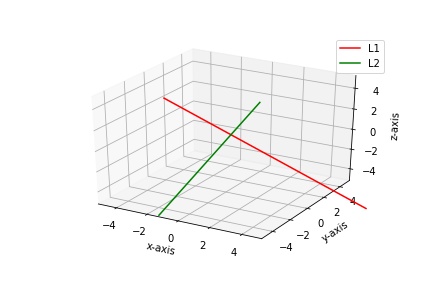
\includegraphics[width=\columnwidth]{lines.png}
	\caption{Lines perpendicular to each other}
	\label{myfig}
\end{figure}\\
\\\end{document}
